\documentclass[
10pt, % Main document font size
letterpaper, % Paper type, use 'letterpaper' for US Letter paper
oneside, % One page layout (no page indentation)
%twoside, % Two page layout (page indentation for binding and different headers)
headinclude,footinclude, % Extra spacing for the header and footer
BCOR5mm, % Binding correction
]{scrartcl}

% my structure and syntax highlighting
\usepackage{mike}
% include image package and the images folder
\usepackage{graphicx}
\graphicspath{ {Diagrams/} }

%----------------------------------------------------------------------------------------
%	TITLE AND AUTHOR(S)
%----------------------------------------------------------------------------------------

\title{\normalfont\spacedallcaps{Bi-Directional JMS Bridge}} % The article title

\author{\spacedlowsmallcaps{Michael Meding* , mikeymeding@gmail.com}} % The article author(s) - author affiliations need to be specified in the AUTHOR AFFILIATIONS block

\date{} % An optional date to appear under the author(s)

%----------------------------------------------------------------------------------------

\begin{document}

\maketitle % Print the title and abstract box

\setcounter{tocdepth}{2} % Set the depth of the table of contents to show sections and subsections only

\tableofcontents % Print the contents section

\thispagestyle{empty} % Removes page numbering from the first page

%----------------------------------------------------------------------------------------
%	ARTICLE CONTENTS
%----------------------------------------------------------------------------------------
 
\section*{Abstract}
This article details the steps involved in creating a bi-directional message bridge between two applications using JMS and HornetQ. For this implementation I used Wildfly as my Java application server but you could use Glassfish or simalar and the implementation would be near identical. Additionally, I assume that the reader of this article has prior knowledge of Java EE 7, EJB, RESTful web services, ActiveMQ and Wildfly application servers. If help is needed setting up any of these items please see the reference section.


 %------------------------------------------------

\section{Overview}

%------------------------------------------------


~\newline

\begin{figure}[h]
\centering
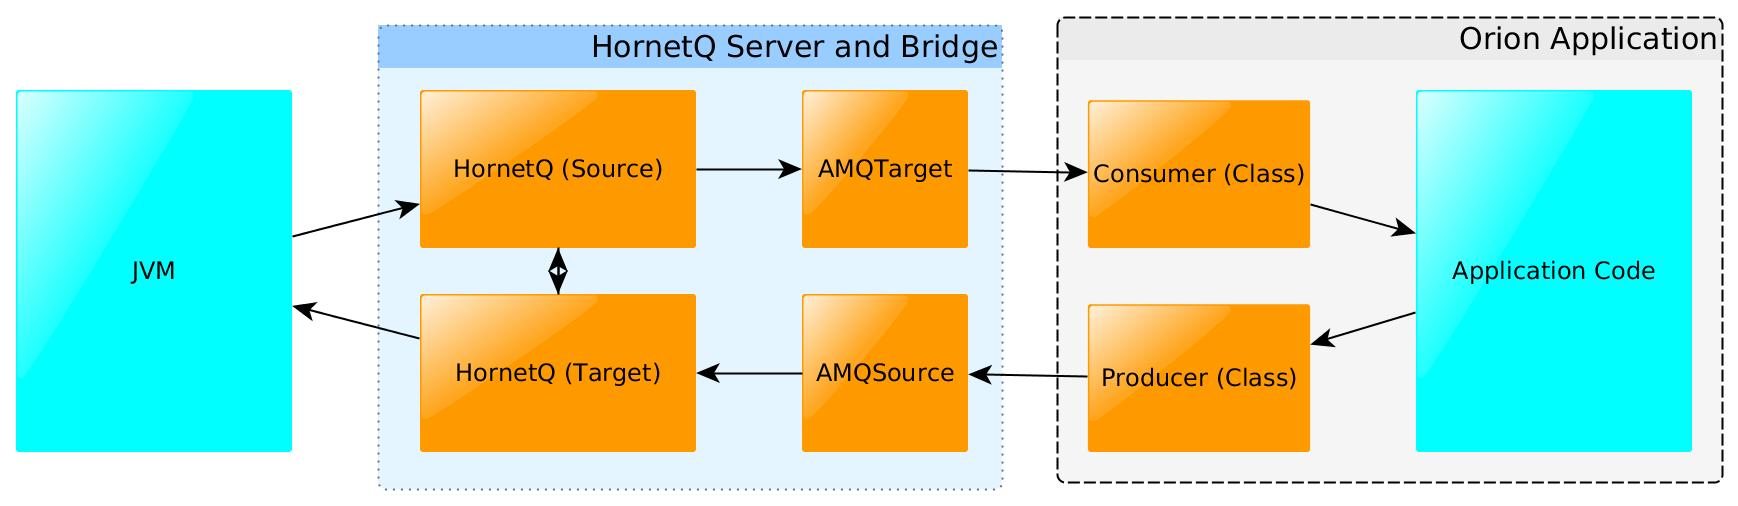
\includegraphics[width=15.5cm]{FlowchartPic} % FLOWCHART
\caption{Two message bridges that provide bidirectional flow of data between the two applications }
\label{fig:servers}
\end{figure}

\begin{figure}[h]
\centering
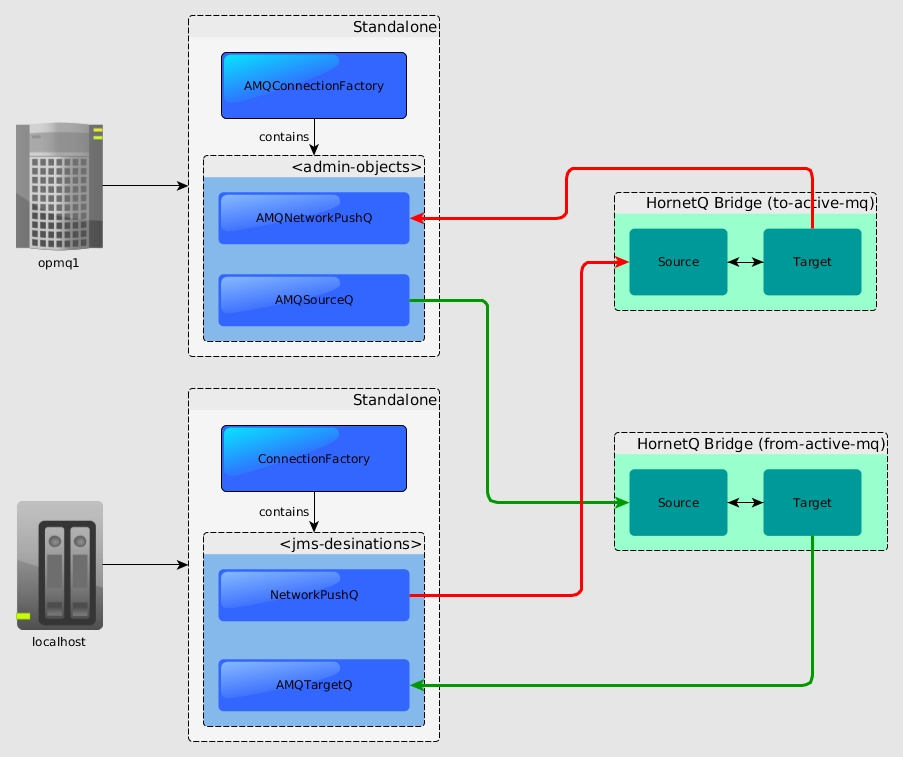
\includegraphics[width=15.5cm]{ConnectionDiagram} % Connection Diagram\textsf{}
\caption{A routing diagram showing a remote JMS setup using HornetQ}
\label{fig:connections}
\end{figure}


\paragraph{}~\newline
As shown by the diagram above HornetQ and bridge definitions are contained in wildfly configuration. The orion application simply includes two classes to communicate back and forth across the two bridges. Messages are managed by ActiveMQ. ActiveMQ is included as an additional module to wildfly and can be accessed by a web console at localhost:61616 when deployed with default settings.

%------------------------------------------------

\section{Setup Wildfly Application Server}

%------------------------------------------------

%Code Snippet
\lstsetxml
\begin{lstlisting}[language=XML]
<!-- placed in the <hornetq-server> definition -->
<jms-destinations>
	<jms-queue name="JMSBridgeSourceQueue">
		<entry name="java:/queue/JMSBridgeSourceQ"/>
		<entry name="java:jboss/exported/jms/queue/JMSBridgeSourceQ"/>
		<durable>true</durable>
	</jms-queue>
	<jms-queue name="AMQTargetQ">
		<entry name="java:/queue/AMQTargetQ"/>
		<entry name="java:jboss/exported/jms/queue/AMQTargetQ"/>
		<durable>true</durable>
	</jms-queue>
</jms-destinations>

<!-- Added after the <hornetq-server> definition -->

<!-- The forward bridge -->
<jms-bridge name="to-active-mq">
	<source>
		<connection-factory name="ConnectionFactory"/>
		<destination name="queue/JMSBridgeSourceQ"/>
	</source>
	<target>
		<connection-factory name="AMQConnectionFactory"/>
		<destination name="queue/JMSBridgeTargetQ"/>
	</target>
	<quality-of-service>AT_MOST_ONCE</quality-of-service>
	<failure-retry-interval>1000</failure-retry-interval>
	<max-retries>-1</max-retries>
	<max-batch-size>10</max-batch-size>
	<max-batch-time>100</max-batch-time>
</jms-bridge>
<!-- The return bridge -->
<jms-bridge name="from-active-mq">
	<source>
		<connection-factory name="AMQConnectionFactory"/>
		<destination name="queue/AMQSourceQ"/>
	</source>
	<target>
		<connection-factory name="ConnectionFactory"/>
		<destination name="queue/AMQTargetQ"/>
	</target>
	<quality-of-service>AT_MOST_ONCE</quality-of-service>
	<failure-retry-interval>1000</failure-retry-interval>
	<max-retries>-1</max-retries>
	<max-batch-size>10</max-batch-size>
	<max-batch-time>100</max-batch-time>
</jms-bridge>
}
\end{lstlisting}

\paragraph{standalone-full.xml} ~\newline\newline
This file is the standard configuration file of the Wildfly application server. For this to work properly you must add the HornetQ module to Wildfly before modifying the standalone-full.xml. Instructions to do this can be found easily on-line. The modifications that must be added for a bi-directional bridge are detailed below. The names given are arbitrary and can be whatever you would like. Throughout this article I follow a pattern of names using source as my origin and target as the endpoint. I would advise following a similar pattern as it begins to get confusing when trying to determine the path of a message. Also keep in mind that the names in jms-destinations must match those in jms-bridge.\newline


%------------------------------------------------

\section{Setup Remote Wildfly Application Server}

%------------------------------------------------

%Code Snippet
\lstsetxml
\begin{lstlisting}[language=XML]
<resource-adapter id="activemq-rar.rar">
	<module slot="main" id="org.apache.activemq"/>
	<transaction-support>NoTransaction</transaction-support>
	<config-property name="ServerUrl">
		tcp://opmq1.outsmartinc.com:61616 <!-- this address must match that of your remote setup -->
	</config-property>
	<connection-definitions>
		<connection-definition class-name="org.apache.activemq.ra.ActiveMQManagedConnectionFactory" jndi-name="java:/AMQConnectionFactory" enabled="true" use-java-context="true" pool-name="AMQConnectionFactory"/>
	</connection-definitions>
	<!-- These are the actual remote queue definitions -->
	<admin-objects>
		<admin-object class-name="org.apache.activemq.command.ActiveMQQueue" jndi-name="queue/BackupSourceQ" use-java-context="true" pool-name="target_queue">
		<config-property name="PhysicalName">
			BackupSourceQueue
		</config-property>
		</admin-object>
	</admin-objects>
</resource-adapter>
\end{lstlisting}

\paragraph{standalone-full.xml} ~\newline\newline
If you wish to read from a remote queue you must include the above resource adapter with a correct tcp pointer to that server. This gets resolved when you start the server so any connection issues will be spit out into the standalone/log/server.log file. In addition the admin objects will be those that exist or will exist on the remote server. These are the queue(s) that you will be speaking to and become either the source or target side of your HornetQ bridge definition.


%------------------------------------------------

\section{JVM Code}

%------------------------------------------------

\subsection {\textbf{Incomming Side (To JVM)}}

\lstsetjava
\begin{lstlisting}[language=Java]
@MessageDriven(activationConfig = {
// these names must match
    @ActivationConfigProperty(propertyName = "destination", propertyValue = "java:jboss/exported/jms/queue/AMQTargetQ"),
    @ActivationConfigProperty(propertyName = "destinationType", propertyValue = "javax.jms.Queue"),
    @ActivationConfigProperty(propertyName = "useJNDI", propertyValue = "true"),
    @ActivationConfigProperty(propertyName = "acknowledgeMode", propertyValue = "Auto-acknowledge")
})

public class MessageReceiverAsync implements MessageListener {

    @Override
    public void onMessage(Message message) {
        try {
            TextMessage tm = (TextMessage) message;
            System.out.println("Message received: " + tm.getText());
        } catch (JMSException ex) {
            Logger.getLogger(MessageReceiverAsync.class.getName()).log(Level.SEVERE, null, ex);
        }
    }
}
\end{lstlisting}

\paragraph{}
This code implements a listener that as soon as a message is posted to AMQTargetQ  (the return bridge) it takes that message and simply prints it out to console. This code runs on the JVM side according to the first diagram above and must be implemented within an EJB to function properly.

%------------------------------------------------

\subsection{\textbf{Outgoing Side (From JVM)}}

\lstsetjava
\begin{lstlisting}[language=Java]
@Stateless
public class MessageSender {

    @Inject
    @JMSConnectionFactory("java:comp/DefaultJMSConnectionFactory")
    JMSContext context;

    @Resource(mappedName = "java:jboss/exported/jms/queue/JMSBridgeSourceQ")
    Queue queue;

    public void sendMessage(String message) {
        context.createProducer().send(queue, message);
    }
}
\end{lstlisting}

\paragraph{}
This is quite straightforward code which simply puts the message into the Queue. You must ensure that your factory name matches that in your standalone-full.xml. For this example I simply used the default that came with the module.


%------------------------------------------------

\section{Application Code}

%------------------------------------------------

\subsection{\textbf{Outgoing Side (Producer)}}


\lstsetjava
\begin{lstlisting}[language=Java]
try {
	// Create a ConnectionFactory
	ActiveMQConnectionFactory connectionFactory = new ActiveMQConnectionFactory("tcp://opmq1.outsmartinc.com:61616");

	// Create a Connection
	Connection connection = connectionFactory.createConnection();
	connection.start();

	// Create a Session
	Session session = connection.createSession(false, Session.AUTO_ACKNOWLEDGE);

	// Create the destination (Topic or Queue)
	Destination destination = session.createQueue("AMQSourceQ");

	// Create a MessageProducer from the Session to the Topic or Queue
	MessageProducer producer = session.createProducer(destination);
	producer.setDeliveryMode(DeliveryMode.PERSISTENT);

	// Create a message
	//String text = "Hello world! From: " + Thread.currentThread().getName() + " : " + this.hashCode();
	String text = "new test message";
	TextMessage message = session.createTextMessage(text);

	// Tell the producer to send the message
	System.out.println("Sent message: " + message.hashCode() + " : " + Thread.currentThread().getName());
	producer.send(message);

	// Clean up
	session.close();
	connection.close();
	
} catch (Exception e) {
	System.out.println("Caught: " + e);
	e.printStackTrace();
}
\end{lstlisting}

\paragraph{}
The pattern for both the producer and consumer are quite similar. Once you have a handle on the queue you just push or pull a message from it.

\subsection{\textbf{Incomming Side (Consumer)}}
\lstsetjava
\begin{lstlisting}[language=Java]
try {
	// Create a ConnectionFactory
	ActiveMQConnectionFactory connectionFactory = new ActiveMQConnectionFactory("tcp://opmq1.outsmartinc.com:61616");

	// Create a Connection
	Connection connection = connectionFactory.createConnection();
	connection.start();

	// Create a Session
	Session session = connection.createSession(false, Session.AUTO_ACKNOWLEDGE);

	// Create the destination (Topic or Queue)
	Destination destination = session.createQueue("JMSBridgeTargetQ");

	// Create a MessageConsumer from the Session to the Topic or Queue
	MessageConsumer consumer = session.createConsumer(destination);

	// Wait for a message
	Message message = consumer.receive(1000);

	if (message instanceof TextMessage) {
		TextMessage textMessage = (TextMessage) message;
		String text = textMessage.getText();
		System.out.println("Received: " + text);
	} else {
		System.out.println("Received: " + message);
	}

	consumer.close();	
	session.close();
	connection.close();
	
	} catch (Exception e) {
		System.out.println("Caught: " + e);
		e.printStackTrace();
}
\end{lstlisting}


\paragraph{}
This is not a listener like the JVM side was. This will timeout after 1 second although if more time than that is required then something has gone wrong. Be sure to check the ActiveMQ console for message status.


%------------------------------------------------

\section{Reference}

%------------------------------------------------

\begin{enumerate}
\item\href{http://blog.c2b2.co.uk/2014/01/connecting-jboss-wildfly-7-to-activemq.html}{''Connecting jboss to ActiveMQ''}
\item\href{file:standalone-full.xml}{Example wildfly standalone file}
\end{enumerate}



\end{document}
